\documentclass[11pt, letterpaper]{article}

% Fonts and Encoding
\usepackage[utf8]{inputenc}
\usepackage[T1]{fontenc}
\usepackage{lmodern} % High-quality Latin Modern vector font

% Math and Symbols
\usepackage{amsmath, amssymb, amsthm, amsfonts, mathrsfs, mathtools}

% Layout and Geometry
\usepackage{geometry}
\geometry{letterpaper, margin=1in}
\setlength{\parindent}{0pt}
\setlength{\parskip}{0.6em}

% Formatting and Graphics
\usepackage{graphicx, xcolor, enumitem, booktabs, array, tabularx}

% TikZ for Illustrations
\usepackage{tikz}
\usetikzlibrary{arrows.meta, positioning, shapes.geometric, calc, backgrounds, matrix}

% Clickable Links and TOC
\usepackage{hyperref}
\hypersetup{
    colorlinks=true,
    linkcolor=blue,
    filecolor=magenta,      
    urlcolor=cyan,
    pdftitle={Advanced Mathematics Topic},
}

% Theorem Environments
\newtheorem{theorem}{Theorem}[section]
\newtheorem{lemma}[theorem]{Lemma}
\newtheorem{proposition}[theorem]{Proposition}
\newtheorem{corollary}[theorem]{Corollary}
\theoremstyle{definition}
\newtheorem{definition}{Definition}[section]
\newtheorem{axiom}{Axiom}[section]
\newtheorem{example}{Example}[section]
\theoremstyle{remark}
\newtheorem{remark}{Remark}[section]

% Custom Commands (Enforced standard notation)
\newcommand{\R}{\mathbb{R}}
\newcommand{\N}{\mathbb{N}}
\newcommand{\Z}{\mathbb{Z}}
\newcommand{\Q}{\mathbb{Q}}
\newcommand{\E}{\mathbb{E}}
\newcommand{\Prob}{\mathbb{P}}
\newcommand{\F}{\mathcal{F}}

\begin{document}

\title{Comprehensive Problem Set: Inverse Laplace Transforms}
\author{Tashfeen Omran}
\date{\today}
\maketitle

\tableofcontents
\newpage

\section{Concept Checklist \& Question Mapping}

This document contains 30 meticulously crafted problems designed to test every concept, trick, and pitfall associated with Inverse Laplace Transforms, as derived from the source material. 

\renewcommand{\arraystretch}{1.5}
\begin{tabularx}{\textwidth}{>{\raggedright\arraybackslash}X >{\centering\arraybackslash}p{3cm}}
\toprule
\textbf{Concept / Problem Type} & \textbf{Question(s)} \\
\midrule
1. Direct Table Lookups (Powers, Exponentials, Sine, Cosine) & 1, 2, 3, 4 \\
2. First Translation (Shifting) Theorem & 5, 6 \\
3. Completing the Square (Basic) & 7, 8 \\
4. Completing the Square with Numerator Shifting & 9, 10, 11 \\
5. Completing the Square with Leading Coefficients & 12, 13 \\
6. Partial Fractions: Distinct Linear Roots (Heaviside Cover-Up) & 14, 15, 16 \\
7. Partial Fractions: Repeated Linear Roots & 17, 18, 19 \\
8. Partial Fractions: Irreducible Quadratics (Coefficient Matching) & 20, 21, 30 \\
9. Second Translation Theorem (Heaviside Step Function \& Delays) & 22, 23, 24 \\
10. The Convolution Theorem & 25, 26 \\
11. Advanced Diagnostic Testing ("Find the Flaw") & 27, 28 \\
12. Synthesis: Solving ODEs via Transform Inversion & 29 \\
\bottomrule
\end{tabularx}

\newpage

\section{Problem Sets}

\textbf{Problem 1:} Evaluate the inverse Laplace transform: $\displaystyle \mathcal{L}^{-1} \left\{ \frac{5}{s^4} \right\}$.

\textbf{Problem 2:} Evaluate the inverse Laplace transform: $\displaystyle \mathcal{L}^{-1} \left\{ \frac{7}{s-4} \right\}$.

\textbf{Problem 3:} Evaluate the inverse Laplace transform: $\displaystyle \mathcal{L}^{-1} \left\{ \frac{8}{s^2 + 25} \right\}$.

\textbf{Problem 4:} Evaluate the inverse Laplace transform: $\displaystyle \mathcal{L}^{-1} \left\{ \frac{3s}{s^2 + 16} \right\}$.

\textbf{Problem 5:} Evaluate the inverse Laplace transform: $\displaystyle \mathcal{L}^{-1} \left\{ \frac{1}{(s-2)^5} \right\}$.

\textbf{Problem 6:} Evaluate the inverse Laplace transform: $\displaystyle \mathcal{L}^{-1} \left\{ \frac{s+3}{(s+3)^2 + 36} \right\}$.

\textbf{Problem 7:} Evaluate the inverse Laplace transform: $\displaystyle \mathcal{L}^{-1} \left\{ \frac{1}{s^2 + 6s + 13} \right\}$.

\textbf{Problem 8:} Evaluate the inverse Laplace transform: $\displaystyle \mathcal{L}^{-1} \left\{ \frac{5}{s^2 - 4s + 29} \right\}$.

\textbf{Problem 9:} Evaluate the inverse Laplace transform: $\displaystyle \mathcal{L}^{-1} \left\{ \frac{s}{s^2 + 8s + 25} \right\}$.

\textbf{Problem 10:} Evaluate the inverse Laplace transform: $\displaystyle \mathcal{L}^{-1} \left\{ \frac{2s - 3}{s^2 - 2s + 10} \right\}$.

\textbf{Problem 11:} Evaluate the inverse Laplace transform: $\displaystyle \mathcal{L}^{-1} \left\{ \frac{4s + 1}{s^2 + 10s + 34} \right\}$.

\textbf{Problem 12:} Evaluate the inverse Laplace transform: $\displaystyle \mathcal{L}^{-1} \left\{ \frac{1}{2s^2 + 8s + 14} \right\}$.

\textbf{Problem 13:} Evaluate the inverse Laplace transform: $\displaystyle \mathcal{L}^{-1} \left\{ \frac{s - 2}{9s^2 + 18s + 18} \right\}$.

\textbf{Problem 14:} Evaluate the inverse Laplace transform: $\displaystyle \mathcal{L}^{-1} \left\{ \frac{3s + 1}{(s-1)(s+2)} \right\}$.

\textbf{Problem 15:} Evaluate the inverse Laplace transform: $\displaystyle \mathcal{L}^{-1} \left\{ \frac{s^2 + 2s + 3}{s(s-2)(s+3)} \right\}$.

\textbf{Problem 16:} Evaluate the inverse Laplace transform: $\displaystyle \mathcal{L}^{-1} \left\{ \frac{5s - 2}{s^2 - 4} \right\}$.

\textbf{Problem 17:} Evaluate the inverse Laplace transform: $\displaystyle \mathcal{L}^{-1} \left\{ \frac{2s + 5}{(s-3)^2} \right\}$.

\textbf{Problem 18:} Evaluate the inverse Laplace transform: $\displaystyle \mathcal{L}^{-1} \left\{ \frac{s^2 - s + 1}{(s+1)^3} \right\}$.

\textbf{Problem 19:} Evaluate the inverse Laplace transform: $\displaystyle \mathcal{L}^{-1} \left\{ \frac{4}{(s-1)^2(s+2)} \right\}$.

\textbf{Problem 20:} Evaluate the inverse Laplace transform: $\displaystyle \mathcal{L}^{-1} \left\{ \frac{3s^2 + 2s + 5}{(s-1)(s^2 + 4)} \right\}$.

\textbf{Problem 21:} Evaluate the inverse Laplace transform: $\displaystyle \mathcal{L}^{-1} \left\{ \frac{s + 7}{(s+2)(s^2 + 2s + 5)} \right\}$.

\textbf{Problem 22:} Evaluate the inverse Laplace transform: $\displaystyle \mathcal{L}^{-1} \left\{ \frac{e^{-2s}}{s^3} \right\}$.

\textbf{Problem 23:} Evaluate the inverse Laplace transform: $\displaystyle \mathcal{L}^{-1} \left\{ \frac{s e^{-4s}}{s^2 + 9} \right\}$.

\textbf{Problem 24:} Evaluate the inverse Laplace transform: $\displaystyle \mathcal{L}^{-1} \left\{ \frac{e^{-s}}{(s-3)^2} \right\}$.

\textbf{Problem 25:} Use the Convolution Theorem to evaluate: $\displaystyle \mathcal{L}^{-1} \left\{ \frac{1}{s(s^2+4)} \right\}$.

\textbf{Problem 26:} Use the Convolution Theorem to evaluate: $\displaystyle \mathcal{L}^{-1} \left\{ \frac{1}{(s^2+1)^2} \right\}$.

\textbf{Problem 27:} \textbf{Find the Flaw:} A student evaluates $\displaystyle \mathcal{L}^{-1} \left\{ \frac{1}{s^2 + 4s + 5} \right\}$. They complete the square to get $(s+2)^2 + 1$. They conclude the answer is $e^{-2t}\cos(t)$. Find the flaw and correct it.

\textbf{Problem 28:} \textbf{Find the Flaw:} A student evaluates $\displaystyle \mathcal{L}^{-1} \left\{ \frac{s}{(s-3)^2 + 16} \right\}$. They state that because the denominator is shifted by $3$, the answer is $e^{3t}\cos(4t)$. Find the flaw and correct it.

\textbf{Problem 29:} Solve the algebraic equation for $F(s)$ and find $f(t)$: $\displaystyle s^2 F(s) - 4F(s) = \frac{1}{s+1}$.

\textbf{Problem 30:} Evaluate the inverse Laplace transform: $\displaystyle \mathcal{L}^{-1} \left\{ \frac{2s^3 + s^2 + 8s + 6}{(s^2+1)(s^2+4)} \right\}$.

\newpage

\section{Detailed Solutions}

\textbf{Problem 1:} Evaluate the inverse Laplace transform: $\displaystyle \mathcal{L}^{-1} \left\{ \frac{5}{s^4} \right\}$.

\textbf{Solution:} 
We use the power rule: $\mathcal{L}\{t^n\} = \frac{n!}{s^{n+1}}$. Here, $n+1 = 4 \implies n = 3$. We need $3! = 6$ in the numerator.
\[
\mathcal{L}^{-1} \left\{ \frac{5}{s^4} \right\} = 5 \cdot \frac{1}{3!} \mathcal{L}^{-1} \left\{ \frac{3!}{s^4} \right\} = \frac{5}{6} t^3
\]
\textbf{Final Answer:} $\displaystyle \frac{5}{6} t^3$

\vspace{1em}

\textbf{Problem 2:} Evaluate the inverse Laplace transform: $\displaystyle \mathcal{L}^{-1} \left\{ \frac{7}{s-4} \right\}$.

\textbf{Solution:}
We use the exponential rule: $\mathcal{L}\{e^{at}\} = \frac{1}{s-a}$. Here, $a = 4$.
\[
\mathcal{L}^{-1} \left\{ \frac{7}{s-4} \right\} = 7 \mathcal{L}^{-1} \left\{ \frac{1}{s-4} \right\} = 7e^{4t}
\]
\textbf{Final Answer:} $\displaystyle 7e^{4t}$

\vspace{1em}

\textbf{Problem 3:} Evaluate the inverse Laplace transform: $\displaystyle \mathcal{L}^{-1} \left\{ \frac{8}{s^2 + 25} \right\}$.

\textbf{Solution:}
We recognize the sine transform: $\mathcal{L}\{\sin(bt)\} = \frac{b}{s^2+b^2}$. Here, $b^2 = 25 \implies b = 5$. We need a $5$ in the numerator.
\[
\mathcal{L}^{-1} \left\{ \frac{8}{s^2 + 25} \right\} = \frac{8}{5} \mathcal{L}^{-1} \left\{ \frac{5}{s^2 + 25} \right\} = \frac{8}{5} \sin(5t)
\]
\textbf{Final Answer:} $\displaystyle \frac{8}{5} \sin(5t)$

\vspace{1em}

\textbf{Problem 4:} Evaluate the inverse Laplace transform: $\displaystyle \mathcal{L}^{-1} \left\{ \frac{3s}{s^2 + 16} \right\}$.

\textbf{Solution:}
We recognize the cosine transform: $\mathcal{L}\{\cos(bt)\} = \frac{s}{s^2+b^2}$. Here, $b^2 = 16 \implies b = 4$.
\[
\mathcal{L}^{-1} \left\{ \frac{3s}{s^2 + 16} \right\} = 3 \mathcal{L}^{-1} \left\{ \frac{s}{s^2 + 16} \right\} = 3 \cos(4t)
\]
\textbf{Final Answer:} $\displaystyle 3 \cos(4t)$

\vspace{1em}

\textbf{Problem 5:} Evaluate the inverse Laplace transform: $\displaystyle \mathcal{L}^{-1} \left\{ \frac{1}{(s-2)^5} \right\}$.

\textbf{Solution:}
Using the First Translation Theorem $\mathcal{L}^{-1}\{F(s-a)\} = e^{at}f(t)$. The base function is $F(s) = \frac{1}{s^5}$, which corresponds to $n=4$. We need $4! = 24$ in the numerator.
\[
\mathcal{L}^{-1} \left\{ \frac{1}{(s-2)^5} \right\} = \frac{1}{24} \mathcal{L}^{-1} \left\{ \frac{4!}{(s-2)^5} \right\} = \frac{1}{24} t^4 e^{2t}
\]
\textbf{Final Answer:} $\displaystyle \frac{1}{24} t^4 e^{2t}$

\vspace{1em}

\textbf{Problem 6:} Evaluate the inverse Laplace transform: $\displaystyle \mathcal{L}^{-1} \left\{ \frac{s+3}{(s+3)^2 + 36} \right\}$.

\textbf{Solution:}
This is a perfectly shifted cosine transform where $a = -3$ and $b = 6$.
\[
\mathcal{L}^{-1} \left\{ \frac{s+3}{(s+3)^2 + 6^2} \right\} = e^{-3t} \cos(6t)
\]
\textbf{Final Answer:} $\displaystyle e^{-3t} \cos(6t)$

\vspace{1em}

\textbf{Problem 7:} Evaluate the inverse Laplace transform: $\displaystyle \mathcal{L}^{-1} \left\{ \frac{1}{s^2 + 6s + 13} \right\}$.

\textbf{Solution:}
The denominator is an irreducible quadratic. We complete the square:
\[
s^2 + 6s + 13 = (s^2 + 6s + 9) + 4 = (s+3)^2 + 2^2
\]
The transform becomes:
\[
\mathcal{L}^{-1} \left\{ \frac{1}{(s+3)^2 + 2^2} \right\} = \frac{1}{2} \mathcal{L}^{-1} \left\{ \frac{2}{(s+3)^2 + 2^2} \right\} = \frac{1}{2} e^{-3t} \sin(2t)
\]
\textbf{Final Answer:} $\displaystyle \frac{1}{2} e^{-3t} \sin(2t)$

\vspace{1em}

\textbf{Problem 8:} Evaluate the inverse Laplace transform: $\displaystyle \mathcal{L}^{-1} \left\{ \frac{5}{s^2 - 4s + 29} \right\}$.

\textbf{Solution:}
Complete the square for the denominator:
\[
s^2 - 4s + 29 = (s^2 - 4s + 4) + 25 = (s-2)^2 + 5^2
\]
The transform is:
\[
\mathcal{L}^{-1} \left\{ \frac{5}{(s-2)^2 + 5^2} \right\} = e^{2t} \sin(5t)
\]
\textbf{Final Answer:} $\displaystyle e^{2t} \sin(5t)$

\vspace{1em}

\textbf{Problem 9:} Evaluate the inverse Laplace transform: $\displaystyle \mathcal{L}^{-1} \left\{ \frac{s}{s^2 + 8s + 25} \right\}$.

\textbf{Solution:}
Complete the square: $s^2 + 8s + 25 = (s+4)^2 + 9$.
We must shift the numerator to match $(s+4)$ using the "Add and Subtract" trick:
\[
s = (s+4) - 4
\]
Substitute this back:
\[
\frac{s}{(s+4)^2 + 3^2} = \frac{s+4}{(s+4)^2 + 3^2} - \frac{4}{(s+4)^2 + 3^2}
\]
Take the inverse transform of each part:
\[
\mathcal{L}^{-1} \left\{ \frac{s+4}{(s+4)^2 + 3^2} \right\} - \frac{4}{3} \mathcal{L}^{-1} \left\{ \frac{3}{(s+4)^2 + 3^2} \right\} = e^{-4t}\cos(3t) - \frac{4}{3}e^{-4t}\sin(3t)
\]
\textbf{Final Answer:} $\displaystyle e^{-4t}\cos(3t) - \frac{4}{3}e^{-4t}\sin(3t)$

\vspace{1em}

\textbf{Problem 10:} Evaluate the inverse Laplace transform: $\displaystyle \mathcal{L}^{-1} \left\{ \frac{2s - 3}{s^2 - 2s + 10} \right\}$.

\textbf{Solution:}
Complete the square: $s^2 - 2s + 10 = (s-1)^2 + 9$.
Rewrite the numerator in terms of $(s-1)$:
\[
2s - 3 = 2(s-1) + 2 - 3 = 2(s-1) - 1
\]
Split the fraction:
\[
\frac{2(s-1) - 1}{(s-1)^2 + 3^2} = 2 \frac{s-1}{(s-1)^2 + 3^2} - \frac{1}{(s-1)^2 + 3^2}
\]
Take the inverse transform:
\[
2e^t\cos(3t) - \frac{1}{3}e^t\sin(3t)
\]
\textbf{Final Answer:} $\displaystyle 2e^t\cos(3t) - \frac{1}{3}e^t\sin(3t)$

\vspace{1em}

\textbf{Problem 11:} Evaluate the inverse Laplace transform: $\displaystyle \mathcal{L}^{-1} \left\{ \frac{4s + 1}{s^2 + 10s + 34} \right\}$.

\textbf{Solution:}
Complete the square: $s^2 + 10s + 34 = (s+5)^2 + 9$.
Rewrite the numerator in terms of $(s+5)$:
\[
4s + 1 = 4(s+5) - 20 + 1 = 4(s+5) - 19
\]
Split the fraction:
\[
\frac{4(s+5) - 19}{(s+5)^2 + 3^2} = 4 \frac{s+5}{(s+5)^2 + 3^2} - \frac{19}{3} \frac{3}{(s+5)^2 + 3^2}
\]
Take the inverse transform:
\[
4e^{-5t}\cos(3t) - \frac{19}{3}e^{-5t}\sin(3t)
\]
\textbf{Final Answer:} $\displaystyle 4e^{-5t}\cos(3t) - \frac{19}{3}e^{-5t}\sin(3t)$

\vspace{1em}

\textbf{Problem 12:} Evaluate the inverse Laplace transform: $\displaystyle \mathcal{L}^{-1} \left\{ \frac{1}{2s^2 + 8s + 14} \right\}$.

\textbf{Solution:}
Factor out the leading coefficient $2$ from the denominator first:
\[
2s^2 + 8s + 14 = 2(s^2 + 4s + 7)
\]
Complete the square inside the parentheses:
\[
s^2 + 4s + 7 = (s+2)^2 + 3
\]
The transform becomes:
\[
\frac{1}{2} \left( \frac{1}{(s+2)^2 + (\sqrt{3})^2} \right)
\]
Multiply and divide by $\sqrt{3}$:
\[
\frac{1}{2\sqrt{3}} \mathcal{L}^{-1} \left\{ \frac{\sqrt{3}}{(s+2)^2 + (\sqrt{3})^2} \right\} = \frac{1}{2\sqrt{3}} e^{-2t} \sin(\sqrt{3}t)
\]
\textbf{Final Answer:} $\displaystyle \frac{1}{2\sqrt{3}} e^{-2t} \sin(\sqrt{3}t)$

\vspace{1em}

\textbf{Problem 13:} Evaluate the inverse Laplace transform: $\displaystyle \mathcal{L}^{-1} \left\{ \frac{s - 2}{9s^2 + 18s + 18} \right\}$.

\textbf{Solution:}
Factor out the leading $9$:
\[
9s^2 + 18s + 18 = 9(s^2 + 2s + 2) = 9((s+1)^2 + 1)
\]
Rewrite the numerator in terms of $(s+1)$:
\[
s - 2 = (s+1) - 3
\]
Substitute back:
\[
\frac{1}{9} \left( \frac{s+1 - 3}{(s+1)^2 + 1} \right) = \frac{1}{9} \frac{s+1}{(s+1)^2 + 1} - \frac{3}{9} \frac{1}{(s+1)^2 + 1}
\]
Take the inverse transform:
\[
\frac{1}{9} e^{-t} \cos(t) - \frac{1}{3} e^{-t} \sin(t)
\]
\textbf{Final Answer:} $\displaystyle \frac{1}{9} e^{-t} \cos(t) - \frac{1}{3} e^{-t} \sin(t)$

\vspace{1em}

\textbf{Problem 14:} Evaluate the inverse Laplace transform: $\displaystyle \mathcal{L}^{-1} \left\{ \frac{3s + 1}{(s-1)(s+2)} \right\}$.

\textbf{Solution:}
Set up partial fractions for distinct linear roots:
\[
\frac{3s + 1}{(s-1)(s+2)} = \frac{A}{s-1} + \frac{B}{s+2}
\]
Use the Heaviside Cover-Up Method:
\begin{align*}
A &= \left. \frac{3s + 1}{s+2} \right|_{s=1} = \frac{4}{3} \\ \relax
B &= \left. \frac{3s + 1}{s-1} \right|_{s=-2} = \frac{-5}{-3} = \frac{5}{3}
\end{align*}
The expansion is:
\[
F(s) = \frac{4/3}{s-1} + \frac{5/3}{s+2}
\]
Take the inverse transform:
\[
f(t) = \frac{4}{3}e^t + \frac{5}{3}e^{-2t}
\]
\textbf{Final Answer:} $\displaystyle \frac{4}{3}e^t + \frac{5}{3}e^{-2t}$

\vspace{1em}

\textbf{Problem 15:} Evaluate the inverse Laplace transform: $\displaystyle \mathcal{L}^{-1} \left\{ \frac{s^2 + 2s + 3}{s(s-2)(s+3)} \right\}$.

\textbf{Solution:}
Set up partial fractions:
\[
\frac{s^2 + 2s + 3}{s(s-2)(s+3)} = \frac{A}{s} + \frac{B}{s-2} + \frac{C}{s+3}
\]
Use the Heaviside Cover-Up Method:
\begin{align*}
A &= \left. \frac{s^2 + 2s + 3}{(s-2)(s+3)} \right|_{s=0} = \frac{3}{(-2)(3)} = -\frac{1}{2} \\ \relax
B &= \left. \frac{s^2 + 2s + 3}{s(s+3)} \right|_{s=2} = \frac{4 + 4 + 3}{2(5)} = \frac{11}{10} \\ \relax
C &= \left. \frac{s^2 + 2s + 3}{s(s-2)} \right|_{s=-3} = \frac{9 - 6 + 3}{-3(-5)} = \frac{6}{15} = \frac{2}{5}
\end{align*}
The expansion is:
\[
F(s) = -\frac{1/2}{s} + \frac{11/10}{s-2} + \frac{2/5}{s+3}
\]
Take the inverse transform:
\[
f(t) = -\frac{1}{2} + \frac{11}{10}e^{2t} + \frac{2}{5}e^{-3t}
\]
\textbf{Final Answer:} $\displaystyle -\frac{1}{2} + \frac{11}{10}e^{2t} + \frac{2}{5}e^{-3t}$

\vspace{1em}

\textbf{Problem 16:} Evaluate the inverse Laplace transform: $\displaystyle \mathcal{L}^{-1} \left\{ \frac{5s - 2}{s^2 - 4} \right\}$.

\textbf{Solution:}
Factor the difference of squares: $s^2 - 4 = (s-2)(s+2)$.
\[
\frac{5s - 2}{(s-2)(s+2)} = \frac{A}{s-2} + \frac{B}{s+2}
\]
Use the Heaviside Cover-Up Method:
\begin{align*}
A &= \left. \frac{5s - 2}{s+2} \right|_{s=2} = \frac{8}{4} = 2 \\ \relax
B &= \left. \frac{5s - 2}{s-2} \right|_{s=-2} = \frac{-12}{-4} = 3
\end{align*}
The expansion is:
\[
F(s) = \frac{2}{s-2} + \frac{3}{s+2}
\]
Take the inverse transform:
\[
f(t) = 2e^{2t} + 3e^{-2t}
\]
\textbf{Final Answer:} $\displaystyle 2e^{2t} + 3e^{-2t}$

\vspace{1em}

\textbf{Problem 17:} Evaluate the inverse Laplace transform: $\displaystyle \mathcal{L}^{-1} \left\{ \frac{2s + 5}{(s-3)^2} \right\}$.

\textbf{Solution:}
For a repeated root, we can use a quick algebraic manipulation instead of full partial fractions. Rewrite the numerator in terms of $(s-3)$:
\[
2s + 5 = 2(s-3) + 6 + 5 = 2(s-3) + 11
\]
Split the fraction:
\[
\frac{2(s-3) + 11}{(s-3)^2} = \frac{2}{s-3} + \frac{11}{(s-3)^2}
\]
Take the inverse transform (using $\mathcal{L}^{-1}\{\frac{1}{(s-a)^2}\} = te^{at}$):
\[
f(t) = 2e^{3t} + 11te^{3t}
\]
\textbf{Final Answer:} $\displaystyle 2e^{3t} + 11te^{3t}$

\vspace{1em}

\textbf{Problem 18:} Evaluate the inverse Laplace transform: $\displaystyle \mathcal{L}^{-1} \left\{ \frac{s^2 - s + 1}{(s+1)^3} \right\}$.

\textbf{Solution:}
Let $u = s+1 \implies s = u-1$. Substitute this into the numerator to easily find the partial fraction expansion:
\[
s^2 - s + 1 = (u-1)^2 - (u-1) + 1 = u^2 - 2u + 1 - u + 1 + 1 = u^2 - 3u + 3
\]
Substitute back into the fraction:
\[
\frac{u^2 - 3u + 3}{u^3} = \frac{1}{u} - \frac{3}{u^2} + \frac{3}{u^3}
\]
Replace $u$ with $s+1$:
\[
F(s) = \frac{1}{s+1} - \frac{3}{(s+1)^2} + \frac{3}{(s+1)^3}
\]
Take the inverse transform. Note that $\mathcal{L}^{-1}\{\frac{1}{(s+1)^3}\} = \frac{t^2}{2!}e^{-t}$:
\[
f(t) = e^{-t} - 3te^{-t} + \frac{3}{2}t^2e^{-t}
\]
\textbf{Final Answer:} $\displaystyle e^{-t} - 3te^{-t} + \frac{3}{2}t^2e^{-t}$

\vspace{1em}

\textbf{Problem 19:} Evaluate the inverse Laplace transform: $\displaystyle \mathcal{L}^{-1} \left\{ \frac{4}{(s-1)^2(s+2)} \right\}$.

\textbf{Solution:}
Set up partial fractions:
\[
\frac{4}{(s-1)^2(s+2)} = \frac{A}{s-1} + \frac{B}{(s-1)^2} + \frac{C}{s+2}
\]
Use the Heaviside Cover-Up Method for the highest powers:
\begin{align*}
B &= \left. \frac{4}{s+2} \right|_{s=1} = \frac{4}{3} \\ \relax
C &= \left. \frac{4}{(s-1)^2} \right|_{s=-2} = \frac{4}{(-3)^2} = \frac{4}{9}
\end{align*}
To find $A$, pick a convenient value for $s$, say $s=0$:
\[
\frac{4}{(-1)^2(2)} = \frac{A}{-1} + \frac{4/3}{1} + \frac{4/9}{2}
\]
\[
2 = -A + \frac{4}{3} + \frac{2}{9} \implies 2 = -A + \frac{14}{9} \implies A = \frac{14}{9} - \frac{18}{9} = -\frac{4}{9}
\]
The expansion is:
\[
F(s) = -\frac{4/9}{s-1} + \frac{4/3}{(s-1)^2} + \frac{4/9}{s+2}
\]
Take the inverse transform:
\[
f(t) = -\frac{4}{9}e^t + \frac{4}{3}te^t + \frac{4}{9}e^{-2t}
\]
\textbf{Final Answer:} $\displaystyle -\frac{4}{9}e^t + \frac{4}{3}te^t + \frac{4}{9}e^{-2t}$

\vspace{1em}

\textbf{Problem 20:} Evaluate the inverse Laplace transform: $\displaystyle \mathcal{L}^{-1} \left\{ \frac{3s^2 + 2s + 5}{(s-1)(s^2 + 4)} \right\}$.

\textbf{Solution:}
Set up partial fractions with an irreducible quadratic:
\[
\frac{3s^2 + 2s + 5}{(s-1)(s^2 + 4)} = \frac{A}{s-1} + \frac{Bs + C}{s^2 + 4}
\]
Find $A$ using Cover-Up:
\[
A = \left. \frac{3s^2 + 2s + 5}{s^2 + 4} \right|_{s=1} = \frac{3 + 2 + 5}{1 + 4} = \frac{10}{5} = 2
\]
Multiply by the denominator to find $B$ and $C$:
\[
3s^2 + 2s + 5 = 2(s^2 + 4) + (Bs + C)(s-1)
\]
Expand and match coefficients:
\[
3s^2 + 2s + 5 = 2s^2 + 8 + Bs^2 - Bs + Cs - C
\]
$s^2$ terms: $3 = 2 + B \implies B = 1$ \\
$s^0$ terms: $5 = 8 - C \implies C = 3$ \\
The expansion is:
\[
F(s) = \frac{2}{s-1} + \frac{s + 3}{s^2 + 4} = \frac{2}{s-1} + \frac{s}{s^2 + 4} + \frac{3}{s^2 + 4}
\]
Take the inverse transform:
\[
f(t) = 2e^t + \cos(2t) + \frac{3}{2}\sin(2t)
\]
\textbf{Final Answer:} $\displaystyle 2e^t + \cos(2t) + \frac{3}{2}\sin(2t)$

\vspace{1em}

\textbf{Problem 21:} Evaluate the inverse Laplace transform: $\displaystyle \mathcal{L}^{-1} \left\{ \frac{s + 7}{(s+2)(s^2 + 2s + 5)} \right\}$.

\textbf{Solution:}
Set up partial fractions:
\[
\frac{s + 7}{(s+2)(s^2 + 2s + 5)} = \frac{A}{s+2} + \frac{Bs + C}{s^2 + 2s + 5}
\]
Find $A$ using Cover-Up:
\[
A = \left. \frac{s + 7}{s^2 + 2s + 5} \right|_{s=-2} = \frac{5}{4 - 4 + 5} = 1
\]
Multiply by the denominator:
\[
s + 7 = 1(s^2 + 2s + 5) + (Bs + C)(s+2)
\]
Match coefficients: \\
$s^2$ terms: $0 = 1 + B \implies B = -1$ \\
$s^0$ terms: $7 = 5 + 2C \implies 2C = 2 \implies C = 1$ \\
The expansion is:
\[
F(s) = \frac{1}{s+2} + \frac{-s + 1}{s^2 + 2s + 5}
\]
Complete the square for the quadratic: $s^2 + 2s + 5 = (s+1)^2 + 4$.
Rewrite the numerator $-s + 1$ in terms of $(s+1)$:
\[
-s + 1 = -(s+1) + 1 + 1 = -(s+1) + 2
\]
Substitute back:
\[
F(s) = \frac{1}{s+2} - \frac{s+1}{(s+1)^2 + 4} + \frac{2}{(s+1)^2 + 4}
\]
Take the inverse transform:
\[
f(t) = e^{-2t} - e^{-t}\cos(2t) + e^{-t}\sin(2t)
\]
\textbf{Final Answer:} $\displaystyle e^{-2t} - e^{-t}\cos(2t) + e^{-t}\sin(2t)$

\vspace{1em}

\textbf{Problem 22:} Evaluate the inverse Laplace transform: $\displaystyle \mathcal{L}^{-1} \left\{ \frac{e^{-2s}}{s^3} \right\}$.

\textbf{Solution:}
We use the Second Shifting Theorem: $\mathcal{L}^{-1}\{e^{-as}F(s)\} = f(t-a)u(t-a)$.
Step 1: Ignore $e^{-2s}$ temporarily. The inverse of $F(s) = \frac{1}{s^3}$ is $f(t) = \frac{t^2}{2}$.
Step 2: The $e^{-2s}$ indicates a time delay of $a = 2$. Replace every $t$ with $(t-2)$ and multiply by the Heaviside step function $u(t-2)$.
\[
f(t) = \frac{1}{2}(t-2)^2 u(t-2)
\]

\begin{center}
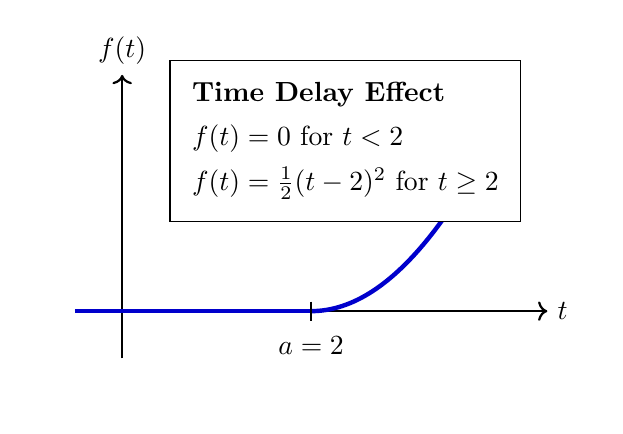
\begin{tikzpicture}[scale=1.2]
    % Background fill to ensure clean rendering
    \fill[white] (-1,-1) rectangle (5,3);
    
    % Axes
    \draw[thick, ->] (-0.5, 0) -- (4.5, 0) node[right] {$t$};
    \draw[thick, ->] (0, -0.5) -- (0, 2.5) node[above] {$f(t)$};
    
    % Plot the delayed function
    \draw[ultra thick, blue!80!black, domain=2:4, samples=50] plot (\x, {0.5*(\x-2)^2});
    \draw[ultra thick, blue!80!black] (-0.5, 0) -- (2, 0);
    
    % Labels and ticks
    \draw[thick] (2, 0.1) -- (2, -0.1) node[below=2pt] {$a=2$};
    
    % Legend Node
    \node[align=left, draw, fill=white, inner sep=8pt, anchor=west] at (0.5, 1.8) {
        \textbf{Time Delay Effect}\\[4pt]
        $f(t) = 0$ for $t < 2$\\[4pt]
        $f(t) = \frac{1}{2}(t-2)^2$ for $t \ge 2$
    };
\end{tikzpicture}
\end{center}

\textbf{Final Answer:} $\displaystyle \frac{1}{2}(t-2)^2 u(t-2)$

\vspace{1em}

\textbf{Problem 23:} Evaluate the inverse Laplace transform: $\displaystyle \mathcal{L}^{-1} \left\{ \frac{s e^{-4s}}{s^2 + 9} \right\}$.

\textbf{Solution:}
Step 1: Ignore $e^{-4s}$. The inverse of $F(s) = \frac{s}{s^2+9}$ is $f(t) = \cos(3t)$.
Step 2: The $e^{-4s}$ indicates a time delay of $a = 4$. Replace $t$ with $(t-4)$ and multiply by $u(t-4)$.
\[
f(t) = \cos(3(t-4)) u(t-4)
\]
\textbf{Final Answer:} $\displaystyle \cos(3(t-4)) u(t-4)$

\vspace{1em}

\textbf{Problem 24:} Evaluate the inverse Laplace transform: $\displaystyle \mathcal{L}^{-1} \left\{ \frac{e^{-s}}{(s-3)^2} \right\}$.

\textbf{Solution:}
Step 1: Ignore $e^{-s}$. The inverse of $F(s) = \frac{1}{(s-3)^2}$ is $f(t) = te^{3t}$ (using the First Shifting Theorem).
Step 2: The $e^{-s}$ indicates a time delay of $a = 1$. Replace every $t$ with $(t-1)$ and multiply by $u(t-1)$.
\[
f(t) = (t-1)e^{3(t-1)} u(t-1)
\]
\textbf{Final Answer:} $\displaystyle (t-1)e^{3(t-1)} u(t-1)$

\vspace{1em}

\textbf{Problem 25:} Use the Convolution Theorem to evaluate: $\displaystyle \mathcal{L}^{-1} \left\{ \frac{1}{s(s^2+4)} \right\}$.

\textbf{Solution:}
The Convolution Theorem states $\mathcal{L}^{-1}\{G(s)H(s)\} = \int_0^t g(\tau)h(t-\tau) \, d\tau$.
Let $G(s) = \frac{1}{s} \implies g(t) = 1$.
Let $H(s) = \frac{1}{s^2+4} \implies h(t) = \frac{1}{2}\sin(2t)$.
The convolution is:
\[
f(t) = \int_0^t 1 \cdot \frac{1}{2}\sin(2\tau) \, d\tau
\]
Evaluate the integral:
\[
f(t) = \frac{1}{2} \left[ -\frac{1}{2}\cos(2\tau) \right]_0^t = -\frac{1}{4}(\cos(2t) - \cos(0)) = \frac{1}{4}(1 - \cos(2t))
\]
\textbf{Final Answer:} $\displaystyle \frac{1}{4}(1 - \cos(2t))$

\vspace{1em}

\textbf{Problem 26:} Use the Convolution Theorem to evaluate: $\displaystyle \mathcal{L}^{-1} \left\{ \frac{1}{(s^2+1)^2} \right\}$.

\textbf{Solution:}
Let $G(s) = \frac{1}{s^2+1} \implies g(t) = \sin(t)$.
Let $H(s) = \frac{1}{s^2+1} \implies h(t) = \sin(t)$.
The convolution is:
\[
f(t) = \int_0^t \sin(\tau)\sin(t-\tau) \, d\tau
\]
Use the trigonometric identity $\sin A \sin B = \frac{1}{2}[\cos(A-B) - \cos(A+B)]$.
Here, $A = \tau$ and $B = t-\tau$.
$A-B = 2\tau - t$ and $A+B = t$.
\[
f(t) = \frac{1}{2} \int_0^t (\cos(2\tau - t) - \cos(t)) \, d\tau
\]
Integrate with respect to $\tau$ (treating $t$ as a constant):
\[
f(t) = \frac{1}{2} \left[ \frac{1}{2}\sin(2\tau - t) - \tau\cos(t) \right]_0^t
\]
Evaluate at the bounds:
Upper bound ($\tau = t$): $\frac{1}{2}\sin(t) - t\cos(t)$
Lower bound ($\tau = 0$): $\frac{1}{2}\sin(-t) - 0 = -\frac{1}{2}\sin(t)$
Subtract the lower bound from the upper bound:
\[
f(t) = \frac{1}{2} \left( \frac{1}{2}\sin(t) - t\cos(t) - \left(-\frac{1}{2}\sin(t)\right) \right) = \frac{1}{2}(\sin(t) - t\cos(t))
\]
\textbf{Final Answer:} $\displaystyle \frac{1}{2}(\sin(t) - t\cos(t))$

\vspace{1em}

\textbf{Problem 27:} \textbf{Find the Flaw:} A student evaluates $\displaystyle \mathcal{L}^{-1} \left\{ \frac{1}{s^2 + 4s + 5} \right\}$. They complete the square to get $(s+2)^2 + 1$. They conclude the answer is $e^{-2t}\cos(t)$. Find the flaw and correct it.

\textbf{Solution:}
\textbf{Flaw:} The student confused the sine and cosine transforms. The cosine transform requires an $s$ (or shifted $s$) in the numerator. Because the numerator is a constant ($1$), this matches the shifted sine transform $\frac{b}{(s-a)^2+b^2}$.
\textbf{Correction:} Here $b=1$, so the numerator is exactly $b$. The correct answer is $e^{-2t}\sin(t)$.

\textbf{Final Answer:} Flaw: Used cosine instead of sine. Correction: $e^{-2t}\sin(t)$.

\vspace{1em}

\textbf{Problem 28:} \textbf{Find the Flaw:} A student evaluates $\displaystyle \mathcal{L}^{-1} \left\{ \frac{s}{(s-3)^2 + 16} \right\}$. They state that because the denominator is shifted by $3$, the answer is $e^{3t}\cos(4t)$. Find the flaw and correct it.

\textbf{Solution:}
\textbf{Flaw:} The student forgot to shift the numerator to match the denominator's $(s-3)$. You cannot apply the First Shifting Theorem unless every $s$ in the function is shifted by the same amount.
\textbf{Correction:} Rewrite the numerator as $s = (s-3) + 3$.
\[
\frac{s-3}{(s-3)^2 + 16} + \frac{3}{(s-3)^2 + 16}
\]
The correct inverse transform is $e^{3t}\cos(4t) + \frac{3}{4}e^{3t}\sin(4t)$.

\textbf{Final Answer:} Flaw: Failed to shift the numerator. Correction: $e^{3t}\cos(4t) + \frac{3}{4}e^{3t}\sin(4t)$.

\vspace{1em}

\textbf{Problem 29:} Solve the algebraic equation for $F(s)$ and find $f(t)$: $\displaystyle s^2 F(s) - 4F(s) = \frac{1}{s+1}$.

\textbf{Solution:}
Factor out $F(s)$:
\[
F(s)(s^2 - 4) = \frac{1}{s+1} \implies F(s) = \frac{1}{(s+1)(s^2-4)} = \frac{1}{(s+1)(s-2)(s+2)}
\]
Set up partial fractions:
\[
\frac{1}{(s+1)(s-2)(s+2)} = \frac{A}{s+1} + \frac{B}{s-2} + \frac{C}{s+2}
\]
Use the Heaviside Cover-Up Method:
\begin{align*}
A &= \left. \frac{1}{(s-2)(s+2)} \right|_{s=-1} = \frac{1}{(-3)(1)} = -\frac{1}{3} \\ \relax
B &= \left. \frac{1}{(s+1)(s+2)} \right|_{s=2} = \frac{1}{(3)(4)} = \frac{1}{12} \\ \relax
C &= \left. \frac{1}{(s+1)(s-2)} \right|_{s=-2} = \frac{1}{(-1)(-4)} = \frac{1}{4}
\end{align*}
The expansion is:
\[
F(s) = -\frac{1/3}{s+1} + \frac{1/12}{s-2} + \frac{1/4}{s+2}
\]
Take the inverse transform:
\[
f(t) = -\frac{1}{3}e^{-t} + \frac{1}{12}e^{2t} + \frac{1}{4}e^{-2t}
\]
\textbf{Final Answer:} $\displaystyle -\frac{1}{3}e^{-t} + \frac{1}{12}e^{2t} + \frac{1}{4}e^{-2t}$

\vspace{1em}

\textbf{Problem 30:} Evaluate the inverse Laplace transform: $\displaystyle \mathcal{L}^{-1} \left\{ \frac{2s^3 + s^2 + 8s + 6}{(s^2+1)(s^2+4)} \right\}$.

\textbf{Solution:}
Set up partial fractions for two irreducible quadratics:
\[
\frac{2s^3 + s^2 + 8s + 6}{(s^2+1)(s^2+4)} = \frac{As + B}{s^2+1} + \frac{Cs + D}{s^2+4}
\]
Multiply by the denominator:
\[
2s^3 + s^2 + 8s + 6 = (As + B)(s^2+4) + (Cs + D)(s^2+1)
\]
Expand the right side:
\[
2s^3 + s^2 + 8s + 6 = As^3 + 4As + Bs^2 + 4B + Cs^3 + Cs + Ds^2 + D
\]
Group by powers of $s$:
\[
2s^3 + s^2 + 8s + 6 = (A+C)s^3 + (B+D)s^2 + (4A+C)s + (4B+D)
\]
Equate coefficients to form a system of equations:
\begin{align*}
s^3&: A + C = 2 \\ \relax
s^2&: B + D = 1 \\ \relax
s^1&: 4A + C = 8 \\ \relax
s^0&: 4B + D = 6
\end{align*}
Solve for $A$ and $C$: Subtract the first equation from the third:
\[
(4A + C) - (A + C) = 8 - 2 \implies 3A = 6 \implies A = 2
\]
Substitute $A=2$ into the first equation: $2 + C = 2 \implies C = 0$.

Solve for $B$ and $D$: Subtract the second equation from the fourth:
\[
(4B + D) - (B + D) = 6 - 1 \implies 3B = 5 \implies B = \frac{5}{3}
\]
Substitute $B=5/3$ into the second equation: $\frac{5}{3} + D = 1 \implies D = -\frac{2}{3}$.

The expansion is:
\[
F(s) = \frac{2s + 5/3}{s^2+1} + \frac{-2/3}{s^2+4} = 2\frac{s}{s^2+1} + \frac{5}{3}\frac{1}{s^2+1} - \frac{2}{3}\frac{1}{s^2+4}
\]
Adjust the last term for the sine transform ($b=2$):
\[
F(s) = 2\frac{s}{s^2+1} + \frac{5}{3}\frac{1}{s^2+1} - \frac{1}{3}\frac{2}{s^2+4}
\]
Take the inverse transform:
\[
f(t) = 2\cos(t) + \frac{5}{3}\sin(t) - \frac{1}{3}\sin(2t)
\]
\textbf{Final Answer:} $\displaystyle 2\cos(t) + \frac{5}{3}\sin(t) - \frac{1}{3}\sin(2t)$

\newpage

\section{Concept Checklist \& Question Mapping (Appendix)}

\renewcommand{\arraystretch}{1.5}
\begin{tabularx}{\textwidth}{>{\raggedright\arraybackslash}X >{\centering\arraybackslash}p{3cm}}
\toprule
\textbf{Concept / Problem Type} & \textbf{Question(s)} \\
\midrule
1. Direct Table Lookups (Powers, Exponentials, Sine, Cosine) & 1, 2, 3, 4 \\
2. First Translation (Shifting) Theorem & 5, 6 \\
3. Completing the Square (Basic) & 7, 8 \\
4. Completing the Square with Numerator Shifting & 9, 10, 11 \\
5. Completing the Square with Leading Coefficients & 12, 13 \\
6. Partial Fractions: Distinct Linear Roots (Heaviside Cover-Up) & 14, 15, 16 \\
7. Partial Fractions: Repeated Linear Roots & 17, 18, 19 \\
8. Partial Fractions: Irreducible Quadratics (Coefficient Matching) & 20, 21, 30 \\
9. Second Translation Theorem (Heaviside Step Function \& Delays) & 22, 23, 24 \\
10. The Convolution Theorem & 25, 26 \\
11. Advanced Diagnostic Testing ("Find the Flaw") & 27, 28 \\
12. Synthesis: Solving ODEs via Transform Inversion & 29 \\
\bottomrule
\end{tabularx}

\end{document}